

\chapter{Functional group-specific traits drive phytoplankton dynamics in the oligotrophic ocean}
\label{chap:4}
\raggedbottom

%\begin{singlespace}
%Harriet Alexander$^{1,2}$, M\'{o}nica Rouco$^3$, Sheean T. Haley$^3$, Samuel T. Wilson$^4$, David M. Karl$^4$, Sonya T. Dyhrman$^{3}$\\
%\\
%$^{1}$ MIT-WHOI Joint Program in Oceanography/Applied Ocean Science and Engineering, Cambridge, MA 02139, USA\\
%$^2$ Biology Department, Woods Hole Oceanographic Institution, Woods Hole, MA 02543, USA\\
%$^3$ Department of Earth and Environmental Sciences Lamont-Doherty Earth Observatory, Columbia University, Palisades, NY 10964\\
%$^4$ Daniel K. Inouye Center for Microbial Oceanography: Research and Education, Department of Oceanography, University of Hawaii, Honolulu, HI 96822, USA\\
%\\
{\let\thefootnote\relax\footnotetext{This chapter was originally published as Alexander, H., R\'{o}uco, M., Haley, S.T., Wilson, S.T., Karl, D.M., and Dyhrman, S.T. (2015). \href{http://www.pnas.org/content/112/44/E5972.full}{Functional group-specific traits drive phytoplankton dynamics in the oligotrophic ocean.} \emph{Proc. Natl. Acad. Sci. U. S. A.} 112:44, E5972-E5979.}}
{\let\thefootnote\relax\footnotetext{H.A. and S.T.D. designed research; H.A., M.R., S.T.H., S.T.W., and S.T.D. performed research; H.A., D.M.K., and S.T.D. analyzed data; H.A. and S.T.D. wrote the paper; and M.R., S.T.H., S.T.W., and D.M.K. contributed to the writing of the paper.}}
{\let\thefootnote\relax\footnotetext{Supplemental Figures, Tables, and Data Sheets for this chapter can be found in \cref{sec:app4}.}}



%\end{singlespace}
\clearpage

\section{Abstract} 
A diverse microbial assemblage in the ocean is responsible for nearly half of global primary production. It has been hypothesized and experimentally demonstrated that nutrient loading can stimulate blooms of large eukaryotic phytoplankton in oligotrophic systems. Although central to better balancing biogeochemical models, knowledge of the metabolic traits that govern the dynamics of these bloom-forming phytoplankton is limited. We employed eukaryotic metatranscriptomic techniques to identify the metabolic basis of functional group-specific traits that may drive the shift between net heterotrophy and autotrophy in the oligotrophic ocean. Replicated blooms were simulated by deep seawater (DSW) addition to mimic nutrient loading in the North Pacific Subtropical Gyre and the transcriptional responses of phytoplankton functional groups were assayed. Responses of the diatom, haptophyte, and dinoflagellate functional groups in simulated blooms were unique, with diatoms and haptophytes significantly (95\% confidence) shifting their quantitative metabolic fingerprint from the \textit{in situ} condition, while dinoflagellates showed little response. Significantly differentially abundant genes identified the importance of co-limitation by nutrients, metals, and vitamins in eukaryotic phytoplankton metabolism and bloom formation in this system. The variable transcript allocation ratio, used to quantify transcript reallocation following DSW amendment, differed for diatoms and haptophytes, reflecting the long-standing paradigm of phytoplankton r- and K-type growth strategies. While the underlying metabolic potential of the large eukaryotic phytoplankton was consistently present, the lack of a bloom during the study period suggests a crucial dependence on physical and biogeochemical forcing, which are susceptible to alteration with changing climate. 
 
\section{Introduction}
It has been postulated that the net oxygen state of oligotrophic systems is controlled by irregular blooms of large eukaryotic phytoplankton \citep{Karl2003}, which have been shown to respond to nutrient input in open ocean ecosystems \citep{McAndrew2007}. Nutrient loading shifts the community away from a tightly regenerating microbial loop, based on small phytoplankton (typically bacterioplankton), towards a community with a higher proportion of larger phytoplankton cells (typically eukaryotic phytoplankton) and, consequently, more carbon export \citep{McAndrew2007}. Data from Station ALOHA in the oligotrophic North Pacific Subtropical Gyre (NPSG) during the summer period have identified increased export of organic carbon, diatom-associated biogenic silica (BSi), and, to a lesser extent, particulate inorganic carbon (PIC) associated with calcification \citep{Karl2012}. These increases are potentially a result of nutrient-driven community shifts. Blooms of eukaryotic phytoplankton in oligotrophic environments are often dominated by the diatom functional group \citep{Villareal2012} and may determine the balance between net heterotrophic and net autotrophic conditions \citep{Karl2003}. Such blooms, however, are thought to be under-sampled and may often go undetected in satellite ocean color records \citep{Villareal2011}. Consequently, the drivers of bloom formation and concomitant carbon export remain poorly understood, particularly in critical oligotrophic systems. \par 
Though central to better balancing global biogeochemical models of GPP \citep{Lopez-Urrutia2006}, knowledge of the biogeochemical drivers that govern the dynamics of these bloom-forming organisms in oligotrophic systems is limited. Nutrient environments are integral to the structuring of phytoplankton communities \citep{Margalef1978, Tilman1977, Cavender-Bares2001} and initiating blooms. Originally thought to be a stable low-fluctuating habitat, long-term monitoring at Station ALOHA has demonstrated that within the constraints of an oligotrophic ecosystem the nutrient regime can be quite dynamic, alternating in controlling factors over many time scales \citep{Karl2001}. These oscillations may be driven by biological (e.g. bloom of N2-fixing cyanobacteria, which draw down P or Fe, while injecting new nitrogen into the system \citep{Karl2002}), physical (e.g. nutrient supply from transient eddies \citep{Benitez-Nelson2007}), or anthropogenic (e.g. atmospheric deposition of nutrients \citep{Kim2014}) forcing.  Regardless of the source, these nutrient-loading events could act to stimulate blooms in the large eukaryotic phytoplankton community.  Historically, the distributions of key eukaryotic phytoplankton function groups have been tracked relative to nutrient stoichiometries to examine how nutrients influence the physiological ecology of different functional groups like diatoms and haptophytes \citep{Cortes2001, Villareal2012}. Although valuable, it is still difficult to relate stoichiometries to the dynamics of bloom formation and, in particular, to patterns in key groups like diatoms without specific measures of functional group physiology. \par
Molecular-level tools that can track transcripts, proteins, or even metabolites and biochemicals in a taxon-specific way are increasingly being employed in cultures and field populations to track metabolic capacity and physiological responses \citep{Marchetti2012a, Alexander2015, Dupont2015, Pearson2015, Ottesen2014, Hennon2015, Dyhrman2012, Amin2015}. Molecular assessment of physiology for eukaryotic populations is most tractable in coastal systems with high biomass \citep{Alexander2015, Dupont2015}, so, in oligotrophic ocean regions, molecular studies of physiology have typically been limited to the numerically abundant members of the microbial community: picoplankton (cyanobacteria, heterotrophic bacteria, and small picoeukaryotes). Groundbreaking studies have demonstrated the responsiveness of the dominant picoplankton community to pulses of deep seawater (DSW) \citep{Shi2012} and of DOM \citep{McCarren2010}, as well as the diel synchrony of the photosynthetic and heterotrophic communities \citep{Ottesen2014}, yet were limited in their coverage of the rare, large eukaryotic fraction due both to the low biomass of their standing stock and the lack of reference sequences. A recent world ocean survey has highlighted the diversity encompassed within the eukaryotic planktonic community \citep{DeVargas2015} and suggested that the structuring of these communities may be driven by physical and chemical oceanographic features \citep{Villar2015}. Yet again, the responsiveness of these keystone eukaryotic phytoplankton communities to changing environmental conditions remains poorly described and understood. 
New resources, including a new marine microbial eukaryote sequencing initiative \citep{Keeling2014}, in combination with the bioinformatic pipeline used here are making possible the study of oligotrophic eukaryotic phytoplankton with unprecedented mechanistic resolution. Here we examined potential biogeochemical controls on phytoplankton bloom formation in the NPSG and the metabolic traits that govern the distribution and responses of unique functional groups. \par

\section{Materials and Methods}
\subsection{Sample collection}
Seawater for the \textit{in situ} eukaryote community mRNA analysis was collected at the HOT, Station ALOHA ($22^\circ 45^\prime$ N, $158^\circ 00^\prime$ W) from a depth of 25 $m$ at 1400 hrs (local time) on three occasions during August and September 2012 as part of the HOE-DYLAN research expedition aboard the R/V Kilo Moana. Hydrocasts for sampling were performed using a conductivity-temperature-depth (CTD) rosette water sampler equipped with 24 Scripps 12-L sampling bottles. Water was collected in acid-washed 20-L carboys and approximately 60-L of seawater was prescreened through $200 \mu m$ mesh and then filtered onto polycarbonate filters ($5.0 \mu m$ pore size, $47 mm$, Whatman) by way of peristaltic pump. This size fraction was targeted to sample large eukaryotic phytoplankton, which are known to form blooms and contribute to export flux in the NPSG. Filters were changed every 20 minutes or when flow rate decreased. Filters were placed in cryovials and stored in liquid nitrogen until mRNA extraction. The total length of filtration time did not exceed 3 hours. Nutrient delivery in the ocean is highly variable; here we chose to model a single nutrient pulse. The incubation experiments were performed with two treatments: a DSW treatment, which included 10\% $0.2 \mu m$ filtered seawater collected from 700 $m$ added to whole seawater collected at 25 m and a control treatment with no addition (\cref{tab:a4t1}). Triplicate 20-L carboys of each treatment were incubated at 30\% surface light levels using on-deck incubators for 7 days and processed as described above on the final day at 1400 h (local time). Nutrient concentrations for phosphate (PO$_4$), nitrate and nitrite [NO$_2$+NO$_3$], and silicate [SiO$_4$] (\cref{tab:a4t1}) were measured by filtering $125mL$ of seawater through a 0.2 $\mu m$, 47-$mm$ polycarbonate filter, and stored frozen ($−20^\circ$C) in acid washed bottles until analysis at the Chesapeake Bay Lab at the University of Maryland according to the facility's protocols. Chlorophyll a was measured on whole water samples collected onto GF\/F filters ($25 mm$, Whatman) using a 90\% acetone extraction and assayed by fluorescence using the AquaFluor Turner TD700 \citep{Parsons1984}. There was little difference between the \textit{in situ} sample and the control treatment both with regards to total chlorophyll a concentration and transcriptional profile (\cref{fig:a4f1,,fig:a4f7}).  There was no significance difference in QMF between the control treatment at the final time point and the \textit{in situ} sample taken at the start of the incubation (\cref{fig:a4f7}). To most conservatively compare non-bloom and bloom scenarios, analyses thus focused on the comparison of the \textit{in situ} community to the DSW amended samples. \par

\subsection{RNA extraction and sequencing}
RNA was extracted from individual filters with the RNeasy Mini Kit (Qiagen), following a modified version of the yeast protocol. Briefly, lysis buffer and RNA-clean zirconia/silica beads was added to the filter and samples were vortexed for 1 minute, placed on ice for 30 seconds, and then vortexed again for 1 minute. Samples were then processed following the yeast protocol. The resulting RNA was eluted in water and then treated for possible DNA contamination using TURBO DNA-free Kit (Ambion) following the Rigorous DNase protocol. RNA from individual filters was then pooled by sample, using the RNA Cleanup Protocol from the RNeasy Mini Kit (Qiagen). The resulting RNA sample thus represented approximately $60 L$ of total seawater for the \textit{in situ} sample. Filters were pooled across like triplicate bottles by treatment, totaling $60 L$ from each of the incubation treatments. The total RNA sample was then enriched for eukaryotic mRNA through a poly-A pull down. The resulting enriched mRNA sample then went through library preparation with the Illumina TruSeq mRNA Prep Kit (Illumina). Libraries were sequenced with the Illumina HiSeq2000 at Columbia Genome Center (New York, NY). Each sample was sequenced to produce a targeted 60 million, 100 base pair, paired end reads. These environmental sequence data are deposited in the Sequence Read Archive (SRA) through the National Center for Biotechnology Information (NCBI) under accession number \href{http://google.com}{SRP056385}. Raw sequence data quality was visualized using FastQC and then cleaned and trimmed using Trimmomatic v 0.27 (paired end mode; 6-base pair wide sliding window for quality below 20; minimum length 25 base pair). \par
\subsection{Genome database creation and mapping}
Environmentally relevant algal genomes (\textit{Aureococcus anophagefferens} CCMP1984 v1.0, \textit{Emiliania huxleyi} CCMP1516 v1.0, \textit{Fragilariopsis cylindrus} CCMP1102 v1.0, \textit{Micromonas pusilla} RCC 299 v3.0, \textit{Ostreococcus lucimarinus} v2.0, \textit{Ostreococcus tauri} v2.0, \textit{Phaeodactylum tricornutum} CCMP632 v2.0, \textit{Pseudo-nitzschia multiseries} CLN-47 v1.0, \textit{Thalassiosira pseudonana} CCMP1335 v3.0) were collected from the Joint Genome Institute \href{http://genome.jgi.doe.gov/}{(JGI) database} and concatenated. Trimmed, paired-end reads from each of the samples were mapped to this concatenated genome library using the Burrows-Wheeler Aligner \citep{Li2010} (BWA-mem, parameters: -k 10 -aM) and then counted using the HTSeq 0.6.1 package \citep{Anders2014}.\par 
\subsection{MMETSP database creation and mapping}
Transcriptome sequences and annotations generated through the Marine Microbial Eukaryote Transcriptome Sequencing Project (MMETSP) that were made public as of 17 March 2014 were collected, representing 401 transcriptomes across 209 species or cultured isolates. Transcriptomes from like species (regardless of strain or condition) and cultured isolates were pooled and clustered using CD-HIT-EST (98\% identity; word size of 9). The resulting clustered set of transcripts was considered to be the representative transcriptome for the species or cultured isolate. Transcriptomes were annotated with KEGG Orthology annotations using the bi-directional best hit (BBH) method through the KEGG Automatic Annotation Server (KAAS) \citep{Moriya2007}. It is worth noting that the KEGG module names are human defined and some genes are artificially grouped in the context of phytoplankton metabolism.  For example, this is the case with the ``methane metabolism'' module, which includes a suite of genes related to carbon not specifically methane metabolism. The 209 transcriptomes created in this manner were concatenated to form a comprehensive species-level transcriptome database from the MMETSP library. Due to the large size of the resulting MMETSP database, trimmed reads were mapped to the MMETSP using the Burrows-Wheeler Aligner \citep{Li2010} (BWA-mem, parameters: -k 10 -aM) and then counted using the HTSeq 0.6.1 package \citep{Anders2014}. \par
\subsection{Differential expression analysis}
Counts obtained from HTSeq were pooled for like-KEGG orthologs across all species in a functional group. The quantitative metabolic fingerprint (QMF) was assessed by normalizing global patterns of expression at the module-level to the total mapped reads, an approach similar to those used in several metagenomic and metatranscriptomic studies focused on prokaryotes \citep{Shi2011, Ottesen2014, Shi2012}. PCA and confidence ellipses of the QMF signals by functional group and sample type (\textit{in situ}, no addition control, and DSW addition) were calculated and visualized using FactorMineR package in R (\cref{fig:c4f2,,fig:a4f7}). No significant difference was seen between the \textit{in situ} and no addition control samples (\cref{fig:a4f7}). For each functional group, the pooled KEGG counts from the \textit{in situ} samples (S1-S3) were compared to those from the corresponding DSW amendment (E1-E3) using Analysis of Sequence Counts (ASC), an empirical Bayes method \citep{Wu2010}. Genes were considered to be differentially abundant between treatments if for a fold change of 2.0 the posterior probability (post-$p$) was greater than 0.95 \citep{Dyhrman2012}. Patterns of differential abundance were visualized using Circos \citep{Krzywinski2009}. Global shifts in the expression of genes independent of functional group were assessed with TMM normalization using the Microbial Assemblage Normalized Transcript Analysis package (MANTA, v. 1.12.0)\citep{Marchetti2012a}. \par
\subsection{Variable transcript allocation modeling} 
Variable transcript allocation following DSW amendment was calculated for each functional group. Though there was a normal distribution of log fold change across all functional groups, the means were off-set for the diatoms and the haptophytes (\cref{fig:a4f4}). From the set of all genes ($G$), the genes which had statistically significant increased transcript abundance (\cref{eq:c4e1}) and decreased transcript abundance (\cref{eq:c4e2}) as identified with ASC (2 fold change, post-$p > 0.95$) \citep{Wu2010} in DSW amended treatments (E) relative to the \textit{in situ} sample (S) were considered. 
%Equation 1 and 2
\begin{equation}
	\label{eq:c4e1}
	 U = \{g : post-p(\frac{T_{E,g}}{T_{S,g}} > 2) > 0.95, g \epsilon G\}
\end{equation}

\begin{equation}
	\label{eq:c4e2}
	 D = \{g : post-p(\frac{T_{S,g}}{T_{E,g}} > 2) > 0.95, g \epsilon G\}
\end{equation}
A variable transcript allocation score ($VTA$) was calculated for both the set of genes with both increased (\cref{eq:c4e3}) and decreased (\cref{eq:c4e4}) abundance, taking the ratio of the summed transcripts per million (T) for the \textit{in situ} (S) and experimental DSW amended treatments (E) of every gene ($u$ or $d$) within the set of significantly differentially abundant genes (U or D). $VTA$ scores were calculated so as to always be greater than one, thus the $VTA_{Dn}$ sums the reciprocal of the ratio summed in $VTA_{Up}$ (\cref{eq:c4e3,,eq:c4e4}). $VTA_{Dn}$ is the magnitude of the decreased transcriptional response following DSW addition, while the $VTA_{Up}$ is the magnitude of the increased transcriptional response following DSW addition. $VTA_{Up}$ and $VTA_{Dn}$, as ratios, focus on the total transcript pool shifted between S and E rather than the number of genes with differential abundance. As such, we can directly compare these two ratios with $VTAR$ (\cref{eq:c4e5}) and assess the metabolic trait of reallocation efficiency. If $VTAR > 1$, there was a larger transcript pool (TPM) in genes that were increased than were decreased, indicating an efficient reallocation of the transcript pool. By contrast, if $VTAR < 1$, less TPM was increased than was decreased. This model defines the total metabolic responsiveness as a trait that can be compared between the functional groups. 
%Equations 3, 4, and 5
\begin{equation}
	\label{eq:c4e3}
	VTA_{Up} = \sum_{u\epsilon U} \frac{T_{E,u}}{T_{S,u}}
\end{equation}
\begin{equation}
	\label{eq:c4e4}
	VTA_{Dn} = \sum_{d\epsilon D} \frac{T_{S,d}}{T_{E,d}}
\end{equation}
\begin{equation}
	\label{eq:c4e5}
	VTAR = \frac{VTA_{Up}}{VTA_{Dn}}
\end{equation}

\section{Results and Discussion}
We leveraged increases in reference sequence availability \citep{Keeling2014} to identify the expressed metabolic capabilities of different phytoplankton functional groups. Total RNA from the eukaryotic community ($>5 \mu m$) of the surface mixed layer at Station ALOHA was sequenced (60 million 100 base pair, poly-A selected, paired end reads) from three samples collected during August-September 2012 (S1-S3). To better understand the underlying functional group-specific metabolism associated with blooms, three blooms were simulated via on-deck incubations. While there are many potential nutrient inputs or bloom drivers (e.g. biologically fixed nitrogen), these blooms were simulated through the addition of deep seawater (DSW) to mimic nutrient loading by upwelling.  These incubation experiments were modeled after \citet{McAndrew2007} and were performed in conjunction with each of the in situ samples, amending surface water with a 10\% mixture by volume of water from below the nutricline (700 m). Sequence reads from the in situ samples (S1-S3) and the bloom simulations (E1-E3) were mapped to 1) non-symbiotic microalgal genomes and 2) a custom database comprised of all publically available transcriptomes as of 17 March 2014 from the Marine Microbial Eukaryotic Transcriptome Project (MMETSP) \citep{Keeling2014}.\par 
The MMETSP provides a 50x expansion of molecular data across the eukaryotic tree of life, which both better reflects the broad diversity within the protists and adds higher-definition coverage for well-studied groups such as diatoms and dinoflagellates \citep{Keeling2014}. Our leveraging of this database for the pipeline developed herein enabled unprecedented identification of taxonomic composition (58-62\% of reads identified) compared to mapping the same dataset to genomes (12-14\%), which have been used in previous studies \citep{Marchetti2012a}. Due to the taxonomic bias of the non-symbiotic algal genomes, the majority of reads from the in situ eukaryote community mRNA samples were annotated as diatoms or haptophytes. When mapped to the custom MMETSP database, however, dinoflagellates dominated, constituting 36-40\% of the mapped reads, with the diatoms and haptophytes the next most highly represented functional groups (\cref{fig:c4f1}A). The dominance of dinoflagellates in the $5 \mu m$ size fraction, confirmed in historic surface pigment analyses at Station ALOHA \citep{Letelier1993}, stands in contrast to previous eukaryotic metatranscriptome studies in the oligotrophic ocean where they accounted for < 5\% of reads \citep{Marchetti2012a}. Although clearly present and important to the community, dinoflagellate read abundance here and in sediment trap data collected during the same cruise series \citep{Fontanez2015} may be magnified by their large transcript pool \citep{Moustafa2010, Hackett2004}. \par

% Figure 1: taxonomic distribution of reads
\begin{figure}[p!]
  \centering
    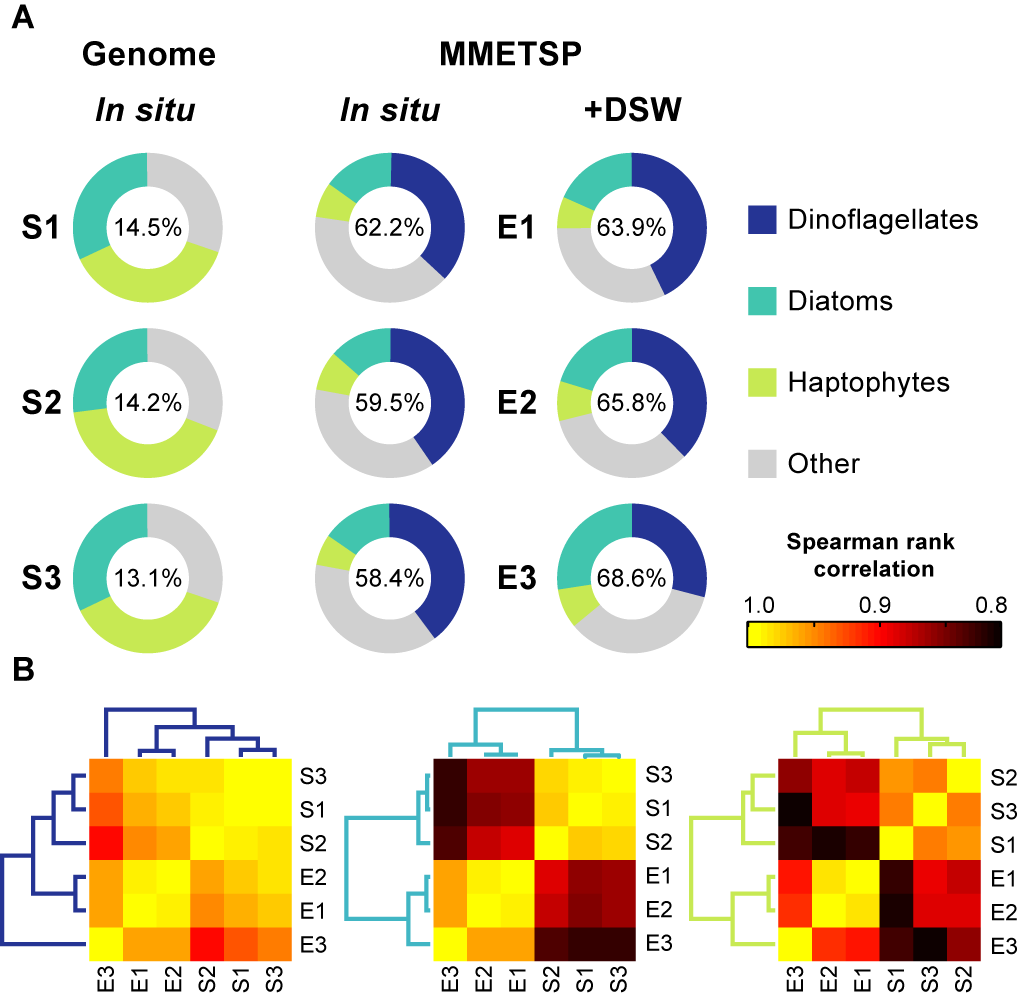
\includegraphics[width=.8\textwidth]{Images/C4_Figure1_Final.png}
    \caption[Taxonomic distribution in mRNA mapped reads consistent across time but altered by deep seawater (DSW) addition]{Taxonomic distribution in mRNA mapped reads consistent across time but altered by deep seawater (DSW) addition. Sequences collected during the summer of 2012 at Station ALOHA (S1: 6 August, S2: 24 August, S3: 2 September) and corresponding deep seawater (DSW) incubation experiments (E1-E3) were mapped to two custom databases: 1) non-symbiotic microalgal genomes and 2) all freely available transcriptomes from the MMETSP as of 17 March 2014. (A) Taxonomic affiliation of reads across the three most abundant functional groups: dinoflagellates, diatoms, and haptophytes mapped to both the genome and MMETSP databases for S1-S3. The corresponding DSW addition incubations E1-E3 were only mapped the MMETSP database. The percent of total reads mapped is indicated inside each of the circles. (B) Spearman rank correlation for species composition shifts within each of the three functional groups across S1-S3 and E1-E3.}
  \label{fig:c4f1}
\end{figure}

The species composition of the functional groups, reflected in rank abundance (\cref{fig:c4f1}B), was highly conserved across all three in situ samples (S1-S3), underscoring the stability of phytoplankton populations in this well-studied oligotrophic system. Between 18.1 and 20.7\% of reads mapped to the MMETSP database were annotated with KEGG orthology, elucidating differences in the mRNA distribution between functional groups at the pathway level. Looking at the module-level, the general distribution of transcripts in proportion to the total was assessed using quantitative metabolic fingerprinting (QMF) \citep{Alexander2015}. Diatoms have a larger proportion of mRNA in the transport-related system (e.g. metallic cation, B12, phosphate, and amino acid) compared to haptophytes and dinoflagellates (\cref{fig:c4f2}A). Purine metabolism was consistently a large component of haptophyte QMF (5.6-27\%), an order of magnitude higher than diatoms and dinoflagellates (1-2\%). Purine nucleotides may represent a source of DON accessible to haptophytes, as haptophytes have been found to grow on purines as their sole N source \citep{Palenik1997}. As the precursors for nucleic acid biosynthesis, purine uptake in the ocean has also been attributed to nucleotide salvage \citep{Winn1984}. These functional group differences observed at the module-level are underscored by principle component analysis (PCA) with the QMF for each functional group differing with 95\% confidence (\cref{fig:c4f2}B) and are suggestive of metabolic partitioning between functional groups. Within a functional group, the QMF was stable across time (\cref{fig:c4f2}A), in contrast to the variability observed in coastal systems over similar time scales \citep{Alexander2015, Dupont2015}. This stability likely reflects both the unique physiological attributes of oligotrophic phytoplankton as well as the comparatively static geochemical environment. \par
%Figure 2. QMF and Circos

\begin{figure}[p!]
  \centerline{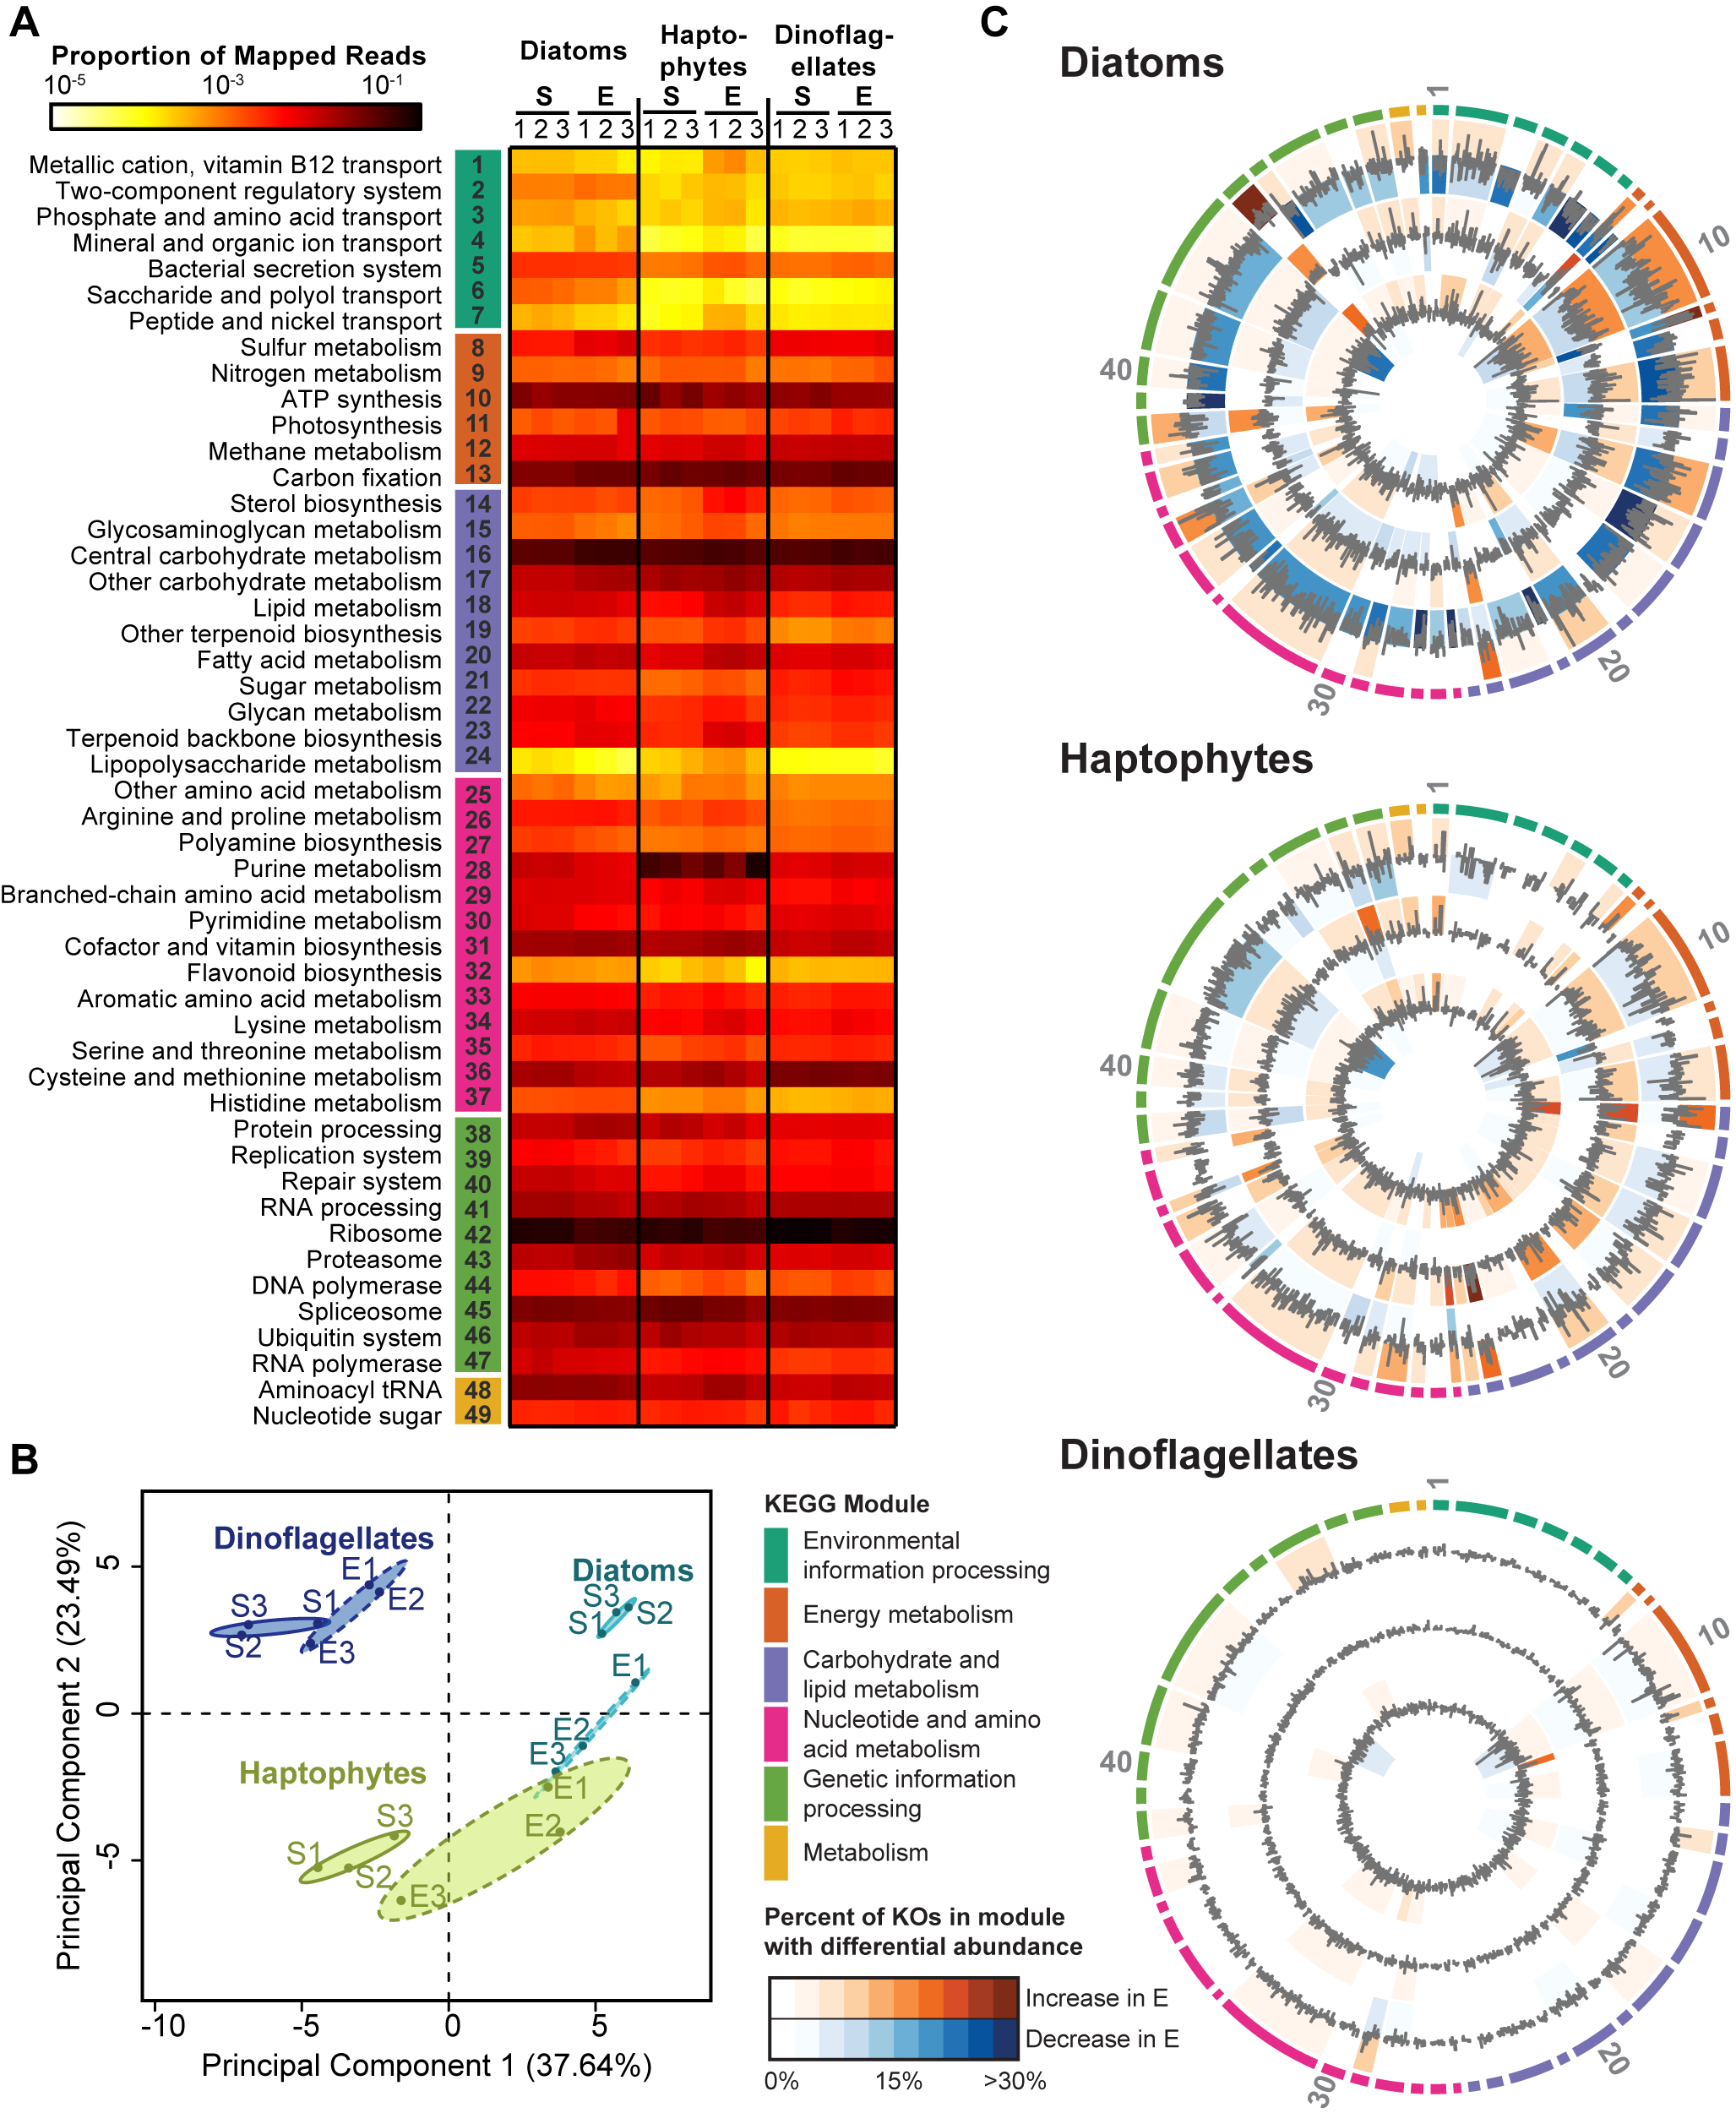
\includegraphics[width=1.1\textwidth]{Images/C4_Figure2_Final.png}}
    \caption[Quantitative metabolic fingerprint (QMF) and patterns of differential expression across KEGG orthology following DSW addition underscore functional group traits]{Quantitative metabolic fingerprint (QMF) and patterns of differential expression across KEGG orthology following DSW addition underscore functional group traits. Caption continued on following page.}
  \label{fig:c4f2}

\end{figure}

\begin{figure}[h!]
    \contcaption{Quantitative metabolic fingerprint (QMF) and patterns of differential expression across KEGG orthology following DSW addition underscore functional group traits. (A) The relative metabolic partitioning of the mRNA pool across the three \textit{in situ} samples (S1-S3) and corresponding deep seawater (DSW) incubation experiments (E1-E3) was assessed using QMF. The summed proportion of mapped reads falling into each of the KEGG modules is depicted as a heat map. (B) Principal component analysis of the QMF signals for each of the functional groups across S1-S3 and E1-E3; 95\% confidence ellipses are indicated for each of the sample types by functional group. (C) Log fold change and significance of differential expression between deep seawater (DSW) amendments and \textit{in situ} samples for KEGG orthologs is visualized with Circos \citep{Krzywinski2009} for the diatoms, haptophytes, and dinoflagellates. Outermost ring colors indicate the KEGG super module, with individual wedges of the pie corresponding to KEGG modules as numbered in A. Concentric circles indicate the expression of the three, replicated DSW addition experiments compared to \textit{in situ} samples: E3 (outer), E2 (middle), E1 (inner). The log fold change of individual KEGG orthologs is depicted as a bar plot bounded -3 to 3. The background color of individual KEGG modules identifies the percentage of genes within module that were significantly (2 fold-change, post-$p > 0.95$) increased (orange) or decreased (blue) in abundance, where darker colors indicate that a higher percentage of genes within that module were significantly different.}
\end{figure}


The static nature of population structure and functional group QMF was altered by replicated nutrient-rich DSW addition experiments, which led to a 7- to 17-fold increase in chlorophyll a, increases not observed in the control treatment (\cref{fig:a4f1}). This increase was consistent with previous studies, which also noted increases in diatoms \citep{McAndrew2007}. Diatom-associated mRNA reads increased in each of the DSW experiments (\cref{fig:c4f1}A). Although species designations can be influenced by the composition of the database used for read mapping, apparent taxonomic shifts occurred at the species-level for diatoms and haptophytes (\cref{fig:a4f2}). Shifts in taxonomic composition were consistent with DSW addition for diatoms and haptophytes, with rank abundance clustering for all experiments (\cref{fig:c4f1}B).  Taxonomic shifts in diatoms were driven by an increase in the rank abundance of certain species, which in all cases were pennate forms (\cref{fig:a4f2}), including genera known to be present in the NPSG like Pseudo-nitzschia \citep{Silver2010} and common in oligotrophic nutrient amendment incubation studies \citep{Marchetti2005, Marchetti2012a}. Although species shifts also occurred within the haptophtyes, \textit{Emiliania huxleyi} was always the most dominant taxon (\cref{fig:a4f2}). The shifts in diatom dominance compared to the consistent dominance of \textit{E. huxleyi} may reflect differences in evolutionary strategies, with metabolic diversity spread across many species in the diatoms and a single species complex with a pangenome, \textit{E. huxleyi}, in the haptophytes \citep{Read2013}. The QMF of DSW addition was significantly different from the QMF of the in situ community for both diatoms and haptophytes, but not dinoflagellates (\cref{fig:c4f2}B). Following DSW addition, the QMF for both diatoms and haptophytes was characterized by increased expression of modules associated with growth, such as carbon fixation (\cref{fig:c4f2}A). These shifts are not the result of changes in species composition, as the patterns of expression from individual species tracked the summed community (\cref{fig:a4f3}). The lack of change in the QMF of dinoflagellates (\cref{fig:c4f2}B) likely reflects their range of life strategies \citep{Hackett2004} and minimal transcriptional regulation of gene expression as observed in culture-studies \citep{Moustafa2010}. \par

%Figure 3

\begin{figure}[h!]
  \centering
    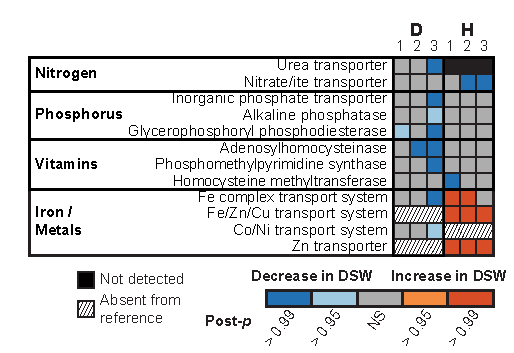
\includegraphics[width=.8\textwidth]{Images/C4_Figure3_Final.pdf}
    \caption[Shifts in transcript abundance of genes responsive to biogeochemical forcing]{Shifts in transcript abundance of genes responsive to biogeochemical forcing. The significance of changes in abundance (2 fold-change, post-$p > 0.95$, or $>0.99$) for genes known to be associated with N, P, vitamin, Fe, or other trace metals metabolism for diatoms (D) or haptophytes (H) is indicated as blue (decrease) or orange (increase). Genes present within the reference transcriptome, but not detected in the field were marked in black, and genes absent from the reference are hashed. KEGG IDs are as follows: Urea transporter (K11959), nitrite/ate transporter (K02575), phosphate transporter (K08176), glycerophosphoryl diester phosphodiesterase (K01126), adenosylhomocysteinase (K01251), phosphomethylpyrimidine synthase (K03147), 5-methyltetrahydrofolate-homocysteine methyltransferase (K00548), iron complex transport system (K02013), iron/zinc/copper transport system (K11706), cobalt/nickel transport system (K02006), zinc transporter (K14715).}
  \label{fig:c4f3}
\end{figure}


Variability within the QMF modules was resolved by statistically assessing the changes in abundance of individual genes for each functional group using a Bayesian approach \citep{Wu2010} (\cref{fig:c4f2,,fig:a4f4}). Statistical significance (2-fold change, posterior probability (post-$p$) > 0.95) of differential abundance was examined for 4038 KEGG orthologs common to diatoms, haptophytes, and dinoflagellates. As with the QMF (\cref{fig:c4f2}A), dinoflagellates demonstrated little to no significant changes in gene expression (\cref{fig:c4f2}C). The suites of transcripts with significantly increased transcript abundance following DSW were highly conserved for both diatoms and haptophytes across the three replicate experiments (40\% of 334 and 19\% of 490 genes common, respectively) but differed between functional groups (41 of the total 824 significantly increased transcripts genes common) (\cref{fig:a4f5}). Of the genes with increased transcript abundance many of those conserved across all three experiments for diatoms and haptophytes were associated with growth (e.g. ATP synthesis (10), photosynthesis (11), and carbon fixation (13)) (\cref{fig:c4f2,,fig:a4f6}). Additionally, following DSW addition, diatoms had signals indicative of the incorporation of both nitrogen (increasing abundance of glutamate and glutamine synthase) and iron (switching from NADPH to ferredoxin sulfate reductase). These changes in transcriptional patterns indicate that both diatoms and haptophytes increase fundamental metabolic processes required for photosynthetic growth in response to DSW. \par
For diatoms and haptophytes, the consistency in genes with increased transcript abundance stands in contrast to the patterns of genes with significantly decreased transcript abundance following DSW addition (\cref{fig:a4f5}). Diatoms were typified by significant decreases in transcript abundance of many genes following DSW, consisting of a large portion (1389 genes) of their metabolism compared to haptophytes (490 genes) (\cref{fig:c4f2}C). Genes with decreased transcript abundance were variable across the three experiments (1.5\% and 6.9\% similar for diatoms and haptophytes, respectively) (\cref{fig:a4f5}) and imply a tailoring of basal metabolism to the change in biogeochemical environment from DSW amendment. Across the KEGG modules, specific genes known to be markers of nutrient limitation significantly decreased in abundance following DSW addition (\cref{fig:c4f3}), potentially signifying a limitation in the in situ population that was alleviated following resupply. Such genes or their protein products are frequently used as proxies to identify limitation in the field \citep{Saito2014}. In E1 and E2, there was a decrease in diatom-associated glycerophosphoryl phosphodiesterase \citep{Dyhrman2012} and adenosylhomocysteinase \citep{Bertrand2012a}, indicative of phosphorus (P) and vitamin limitation, respectively (\cref{fig:c4f3}). Silica transporters, though not in KEGG, were surveyed and not found to have significant shifts in abundance. E3 was characterized by a decrease in abundance of many genes indicative of limitation in the diatoms, including but not limited to, a urea transporter \citep{Bender2012}, a phosphate transporter \citep{Dyhrman2012}, and metal transporters (\cref{fig:c4f3}). This is suggestive of diatom co-limitation in E3, similar to patterns of co-limitation recently observed in picocyanobacteria in the Pacific Ocean \citep{Saito2014}. There was a decrease in transcript abundance for haptophyte-associated nitrate and nitrite transporters in E2 and E3 and homocysteine methyltransferase in E1 (\cref{fig:c4f3}). This may be indicative of nitrogen and vitamin limitation based on the pattern in other organisms \citep{Bertrand2012a, Bender2014}, but the regulation of these targets in haptophytes is poorly understood. Metal transport proteins were significantly increased for haptophtyes in E1-E3 and indicated metabolic strategies following the addition of resources that differ from diatoms. In contrast to the diatoms, no markers of P limitation, such as the phosphate transporter or alkaline phosphatase in \textit{E. huxleyi} \citep{Dyhrman2006, Dyhrman2003, Xu2006}, were significantly decreased for haptophytes, consistent with their known tolerance for P limitation \citep{Lessard2005}. These data evince that diatoms and haptophytes are not under the same biogeochemical controls in situ and employ disparate strategies following DSW addition to capitalize on newly available resources. Being able to identify and characterize multiple markers of limitation in a genera-specific manner for these eukaryotes is of central importance to the modeling of aperiodic blooms of these groups in oligotrophic systems. \par 



%Figure 4
\begin{figure}[p!]
  \centering
    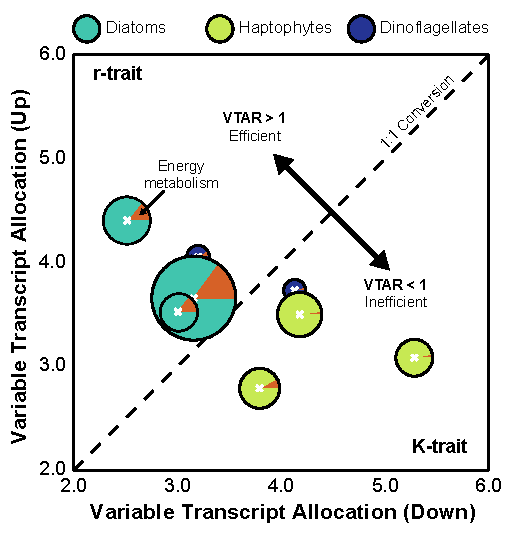
\includegraphics[width=.8\textwidth]{Images/C4_Figure4_Final.pdf}
    \caption[Variable transcript allocation space differentiates functional group strategies]{Variable transcript allocation space differentiates functional group strategies. The variable transcript allocation score (Equations \ref{eq:c4e3} and \ref{eq:c4e4}) of the genes with significantly increased ($VTA_{Up}$) or decreased ($VTA_{Down}$) abundance in the deep seawater (DSW) amendment relative to the \textit{in situ} sample is plotted for diatoms, haptophytes, and dinoflagellates for E1-E3. The size of the pie indicates the total number of genes with significantly different transcript abundances between the \textit{in situ} and DSW amended treatments. The proportion of increased TPM in E within the energy metabolism super group is illustrated as a pie slice in orange.}
  \label{fig:c4f4}
\end{figure}



The above analyses focus primarily on the gene content and transcriptional patterns; however, the underlying eco-evolutionary metabolic traits for a functional group may be better described by considering the shift in the total transcript pool (TPM). Using the statistically resolved patterns of increases and decreases in transcript abundance, a variable transcript allocation ratio ($VTAR$) was calculated to model functional group transcriptional responsiveness to DSW amendment (\cref{fig:c4f4}). $VTAR > 1$ indicates an efficient reallocation of the transcriptional potential from genes with decreased abundance to genes with increased abundance following DSW amendment, while $VTAR < 1$ indicates an inefficient reallocation. The dinoflagellates had variable $VTA$ scores due to their small pool of differentially abundant genes, however the $VTA$ scores consistently resulted in disparate patterns for the diatom and the haptophytes (\cref{fig:c4f4}). In every experiment, the diatoms fell above the 1:1 line, with a $VTAR > 1$ ($1.15 - 1.75$), while haptophytes fell below, with a $VTAR < 1$ ($0.58 - 0.83$) (\cref{fig:c4f4}). The relative efficiency of reallocation, here defined by $VTAR$, reflects differences in the metabolic traits of these functional groups and aligns with preexisting ecological traits as defined by \citep{Margalef1978}. Diatoms are r-selected with high maximum uptake rates that enhance their competition under high or fluctuating nutrients (such as a DSW upwelling event). This trait is reflected in the significant decrease in transcript abundance of many genes across a broad metabolic range coupled with the targeted increase of a subset of genes largely falling within the energy metabolism super module (\cref{fig:c4f4}), a pattern which was also observed with gene-focused analyses using trimmed mean of M value (TMM) normalization \citep{Marchetti2012a, Robinson2010} (\cref{fig:a4f6}). Haptophytes are K-selected, possessing a low half-saturation constant that enhances growth under low nutrient conditions, but are unable to capitalize on nutrient pulses like r-selected competitors. Again, this ecological trait is reflected in changes in the haptophyte transcript pool. Though numerically fewer of their genes significantly decreased in abundance with DSW addition, the total TPM represented by those genes with decreased abundance exceeded that of those induced, defined by $VTAR <1$ (\cref{fig:c4f4}). This is also reinforced by the gene-specific analysis (\cref{fig:a4f6}). It has been speculated that the mechanistic basis for the r- and K- tradeoff dichotomy in the phytoplankton lies in the disparate investment in growth or resource acquisition machinery \citep{Litchman2008}. The large portion of the transcript pool that increased ($VTAR > 1$) for diatoms shows an ability to capitalize on newly available resources, with 14.2-14.9\% of the increased TPM in the KEGG energy metabolism super module (\cref{fig:c4f4}). 
Haptophytes ($VTAR < 1$), by contrast, do not efficiently reallocate the transcript pool, with only 5.5-10.2\% of the increased TPM in energy metabolism (Figure  \ref{fig:c4f4}). In short, haptophytes do not appear to modulate their transcript pool to capitalize on growth processes as efficiently as diatoms (Figure  \ref{fig:c4f4}). \par



These functional group-specific molecular and metabolic mechanisms underpin the aperiodic eukaryotic phytoplankton blooms in the oligotrophic ocean. Whereas both diatoms and haptophytes, including calcifying groups, likely contribute to a shift towards a net autotrophic condition when there is a nutrient pulse, the ecosystem function of oligotrophic systems may ultimately hinge on the unique trait of the diatoms to more efficiently turn over their scavenger metabolism to one of enhanced production. This finding is consistent with the dominance of diatom-associated BSi export relative to PIC export during summer in the NPSG \citep{Karl2012}. Unlike the preceding 13 years of study at Station ALOHA \citep{Karl2012}, enhanced production and export characteristic of bloom events were not observed during the summer of 2012, which exhibited a period of sustained net-heterotrophy. We demonstrated through simulated blooms that the metabolic capacity for enhanced production is inherent in the large eukaryotic phytoplankton regardless of water mass, suggesting that the lack of bloom in 2012 was variably due to deficiency in macronutrients, vitamins, and metals. As the conditions observed during summer 2012 may be increasingly encountered in a future ocean \citep{Doney2012}, modeling the molecular traits and tradeoffs of these populations will help better predict ecosystem state and metabolic balance of the ocean. \par








